% CAPITULO 1: EXPLICO EL ESQUEMA GENERAL DEL ALGORITMO

\chapter{Herramienta desarrollada}
\label{method}


\section{Fundamentos del método utilizado}
\label{fundamentos}
% Mapeo de los objetivos con existencia de herramientas disponibles.

% PRIMERO QUE BUSCAMOS EN REALIDAD
Para entender los fundamentos del método implementado primero debemos analizar mejor los detalles del objetivo.
El requerimiento fundamental de la secuencia linker resultante es que esta posea la flexibilidad necesaria para que los dominios que conecta se muevan libremente.
Para poder lograr esto, tal como se puede deducir de los conceptos visto sobre flexibilidad, la secuencia
debe adoptar \textit{in-vivo} las características de un amplio ensamble conformacional, donde las diferentes conformaciones desordenadas se intercambian rápidamente de manera continua.
Como vimos a lo largo de la introducción, este tipo de conformación es adoptada por las secuencias que caracterizamos como IDRs/IDPs.
% La adopcion de una conformacion intrinsecamente desordenada por parte de la secuencia linker proveerá, entonces, la flexibilidad necesaria por su correcto funcionamiento.
Por lo tanto, tenemos un panorama mas claro acerca de cuales serán las características conformacionales de la secuencia que esperamos obtener.


% Como vimos en la sección \ref{linkerDesign} la flexibilidad no es todo y, por eso, 
Otra parte fundamental del objetivo es que el linker obtenido se mantenga inerte frente a cualquier actividad biológica que pueda 
interferir en el proceso se expresión o en la correcto funcionamiento de la proteína resultante del diseño.
% Una parte relevante de esta secuencia objetivo es su inercia frente al pipeline de 
En la sección \ref{functionalLandscape} se describieron distintos elementos funcionales que pueden estar presentes en una secuencia.
Clasificando, aislando y analizando estos elementos hemos podido comprender mejor cuales son sus propiedades. 
Lo que lo objetivo requiere, entonces, es que la secuencia resultante este libre de cualquiera de estos elementos permaneciendo, preferentemente, inerte ante cualquier actividad o interacción posible \textit{in-vivo}.

% Teniendo en claro los objetivos en términos de los posibles elementos estructurales y funcionales, lo que el método requiere es, entonces, obtener una secuencia que adopte ,que esté limpia de elementos estructurales 
A lo largo del capítulo 1, hemos presentado una gran cantidad de conocimientos obtenidos acerca de las propiedades secuenciales y su relación con la conformación y función resultante.
Los avances mostrados en este campo se trasladan a una gran cantidad(y variedad) de métodos que permiten predecir la ocurrencia de estas propiedades sobre cualquier secuencia polipeptídica.
% De forma abstracta, estas herramientas permiten predecir el mapeo entre la secuencia y el perfil de propiedades resultantes. 
% Diferentes herramientas bioinformáticas resultan de trasladar estos conocimientos a
% Estos avances, además, dieron paso al desarrollo de una gran cantidad(y variedad) de herramientas bioinformáticas que permiten predecir éstas propiedades a partir de la secuencia .
% La disponibilidad de estas herramientas permite tener una idea más clara del comportamiento que tendrá una proteína en un contexto experimental dado, solamente conociendo su secuencia y utilizando las herramientas adecuadas. 
% 
Conociendo en detalle los requerimientos que esperamos para la secuencia resultante
y haciendo uso de este amplio set de herramientas, podemos analizar cualquier secuencia y estimar si estos se cumplen.
Lo que queda saber, entonces, es cómo se llegará a una secuencia que cumpla estas características.


%  ESTO DEBERIA IR EN ALGUN LADO, NO SE DONDE PONERLO
% Por encima de estos requerimientos se aplican las propiedades extras que son parte de las utilidad extra que ayudan a la utilización experimental de las secuencias resultantes.









% Hipótesis asumida respecto del espacio de soluciones, dependencia de la superficie de búsqueda con las propiedades a evaluar.
% *****************PROPIEDADES DEL ESPACIO DE BUSQUEDA 

% COMPLEJIDAD DE LAS IDPs
% SACADO DE A decade and a half of protein intrinsic disorder: Biology still waits for physics
Algunos de los conceptos vistos en el capítulo 1, principalmente con respecto a aspectos conformacionales, pueden ser usados para llegar a una secuencia con las características buscadas.
Se vió que las secuencias caracterizadas como IDRs/IDPs estaban claramente sesgadas en su composición, con baja complejidad y generalmente desprovistas de varios tipos de aminoácidos.
Esto parece indicar que el espacio de secuencias comprendido por éstas debe ser significativamente pequeño.
% It was pointed out that IDPs possess noticeable amino acid biases, and many IDPs/IDPRs are characterized by sequence redundancy and low sequence
% complexity, containing long stretches of various repeats and being completely devoid of some (often many) types of amino acid residues. 
% These observations seem to indicate that the sequence space of IDPs/IDPRs should be simpler than that of ordered proteins.
% However, the reality is more complex than conventional wisdom might suggest, and the sequence space attainable by simple IDPs/IDPRs 
% is more diversified than that of the structurally more sophisticated ordered proteins.

Sin embargo, la complejidad es mucho mayor de lo que parece. 
% En \cite{uversky2013decade} se realiza un análisis más detallado de la esta `simple complejidad' del espacio secuencial asociado a las IDRs/IDPs.
Lo más relevante para nuestra aplicación es que, basándose en los requerimientos estructurales que existen en las regiones/proteinas que adoptan estructuras ordenadas, el espacio de secuencias asociado a éstas es
mucho menor que el correspondiente a las IDRs/IDPs. La falta total o parcial de una estructura ``codificada'' en la secuencia, como se analiza en \cite{uversky2013decade}, 
indica que el tamaño del espacio secuencial que ocupan las IDRs/IDPs(al menos aquellas que nunca logran plegarse, las que estamos buscando) es considerablemente mayor que el 
espacio plegable(aquel que ocupan las secuencias que traen codificada la información necesaria para experimentar plegamiento).

Es decir, el espacio abarcado por las secuencias que poseen las propiedades conformacionales que buscamos, no es tan restringido como se podría pensar y, de hecho,
puede tener un tamaño considerable con respecto al espacio total de posibles soluciones.
% Un polipéptido de unos 100 residuos de longitud con una distribución al azar de AAs abarca un espacio total compuesto por unas $20^{100}$ (aprox. $10^{130}$) secuencias.   
% Obviamente, no todas las secuencias al azar se pliegan para dar una estructura unica y, por lo tanto, no cualquier secuencia pertenecerá al conjunto que denominamos como plegadas.
% Lo que se encuentra es que el espacio ocupado por secuencias plegadas es significativamente menor que el espacio total de secuencias\cite{dill1999polymer}.
% 
% Las secuencias caracterizadas como IDRs/IDPs no necesitan adquirir una estructura ordenada 
% Foldable proteins fold first and then bind to their partners whereas IDPs/IDPRs remain disordered until they interact with their partners. 
% Furthermore, many IDPs/IDPRs do not require folding to be functional, and some of them form fuzzy complexes, in which they preserve significant amount of disorder. 
% All this suggests that the sequence space of IDPs (at least those which either do not fold at all or do not completely fold at binding) 
% is noticeably greater than the “foldable” sequence space due to the removal of restrictions posed by the need to gain ordered structure spontaneously. 
% This represents one of the conundrums of intrinsic disorder, where the apparent sequence redundancy and simplicity are combined with the lack of structural restrains leading to the increase in the dimensions and complexity of the
% available sequence space.


% 
% En los últimos años se han realizado importantes avances en el estudio de las relación existente entre la estructura primaria de proteínas y el conjunto de propiedades experimentalmente observables de éstas(\textit{in-vivo} o \textit{in-vitro}). 

% 
% 
% 
% El problema que estamos enfrentando es, sin embargo, el inverso. Queremos  
% Nuevamente, planteandolo de forma abstracta, esto representa mapear el espacio de comportamientos con el espacio de secuencias posibles.
% 
% Claramente, ambos problemas están íntimamente relacionados: un mejor entendimiento de los principios que hacen posible(y necesarios) para que una secuencia tenga un cierto comportamiento, brindarán mayor información
% It is clear that the two problems are closely related to each other: a better understanding of the principles of protein folding makes it possible to clarify which features of protein sequences are necessary (as well as sufficient) 
% for stability and fast folding; in other words, the features that make a protein a protein. 
% Such understanding focuses the attention of designers on emphasizing these crucial features of folding sequences.
% 
% Obtener una secuencia con un comportamiento muy específico(por ejemplo que adquiera una estructura plegada definida), puede ser un requerimiento muy específico.
% Un reflejo de esto puede verse en las estructuras de ciertas proteinas naturales, las cuales tienen una fuerte dependencia con la secuencia que se mantiene altamente conservada. 
% 
% Sin embargo, como se detalló en la sección previa, el objetivo de nuestra herramienta es lograr obtener una secuencia con un comportamiento bastante 'simple' de obtener.... 







% YA DIJE COMO EVALUAR LOS REQUERIMIENTOS
% YA DIJE COMO ERA EL ESPACIO DE SOLUCIONES
% AHORA
% ************EL MÉTODO
De esta forma, estamos en una situación en la que: tenemos un conjunto de herramientas que nos permiten mapear cada secuencia con distintos comportamientos (deseado o no deseados) de acuerdo a nuestros objetivos y, además, 
podemos asumir que el conjunto de secuencias que cumple con los principales comportamientos buscados es considerablemente grande con respecto al espacio de soluciones posibles (cualquier combinación de AAs).

% El método para buscar la secuencia resultante, 
% de búsqueda dependerá de nuestros objetivos y los conocimientos, desconocimientos, hipotesis acerca del espacio de búsqueda.
Una primera aproximación obvia sería realizar una búsqueda sistematica dentro del espacio de secuencias hasta obtener una que resulte favorable de acuerdo a nuestros parámetros de evaluación.  
% probar distintas combinaciones al azar...
El problema radica en que es una forma totalmente ineficiente de búsqueda, tiene un alto costo computacional y el resultado(asumiendo que lo encontramos) será una composición 
al azar.
Una aproximación mas adecuada, que será detallada en este capítulo, sería utilizar todo el conocimiento que tenemos para poder evaluar la secuencia y usar esto a nuestro favor para guiar la búsqueda. 
Al guiar la búsqueda utilizando los resultados de las evaluaciones, esta sera mucho mas efectiva y el costo computacional sera mucho menor.
Además, según el punto de inicio que utilicemos para la búsqueda, podremos intentar obtener secuencias resultantes con cierta similitud.

% La existencia de una función ideal implicaría que esta represente la dependencia de cada posicion con el contexto de la secuencia, con respecto a la propiedad analizada.
% Si bien las herramientas disponibles de predicción nos son las ideales, generalmente brindan información sobre cada posición y no sobre la secuencia como un todo.

% Uilizando esta información podríamos analizar que posiciones no son acordes con el comportamiento/propiedades deseado/a y utilizar esta información para guiar la búsqueda, modificando solo aquellas posiciones que no nos resultan favorables.
 
% Si bien asumimos que el conjunto de secuencia que cumplen las condiciones estandar del resultado es grande con respecto al especio total de soluciones, no conocemos la forma funcional que no esta guiando la busqueda,
% es decir, como esta depende con la secuencia.  Para implementar un mecanismo eficiente de búsqueda debemos tener en cuenta este desconocimiento.










\section{Esquema general de la implementación}

El procedimiento general del algoritmo consiste en aplicar mutaciones puntuales iterarativamente a partir de una secuencia inicial, en busca de la secuencia final con las características deseadas.
En cada iteración se proponen y analizan posibles mutaciones de acuerdo a un sistema de evaluación de secuencias.
La selección de posibles posiciones a mutar se hace de acuerdo a un muestreo ponderado en función de los resultados de la evaluación secuencial.
Además, la aceptación de cada mutación está asociada a un método heurístico de decisión.
De esta forma, la secuencia de mutaciones aceptadas para una determinada secuencia inicial no necesariamente será siempre la misma, 
la búsqueda será guiada por el análisis realizado sobre las secuencias pero no quedará completamente determinada por éste. 

En la figura \ref{fig:esquema-algoritmo} se ve un esquema general del método completo. 
En la secciones \ref{seqInicial} y \ref{evalYmutacion} se detalla como se obtiene la secuencia inicial y se describen y ejemplifican los pasos para obtener una mutación puntual en cada iteración.


\begin{figure}[h!]
\centering
   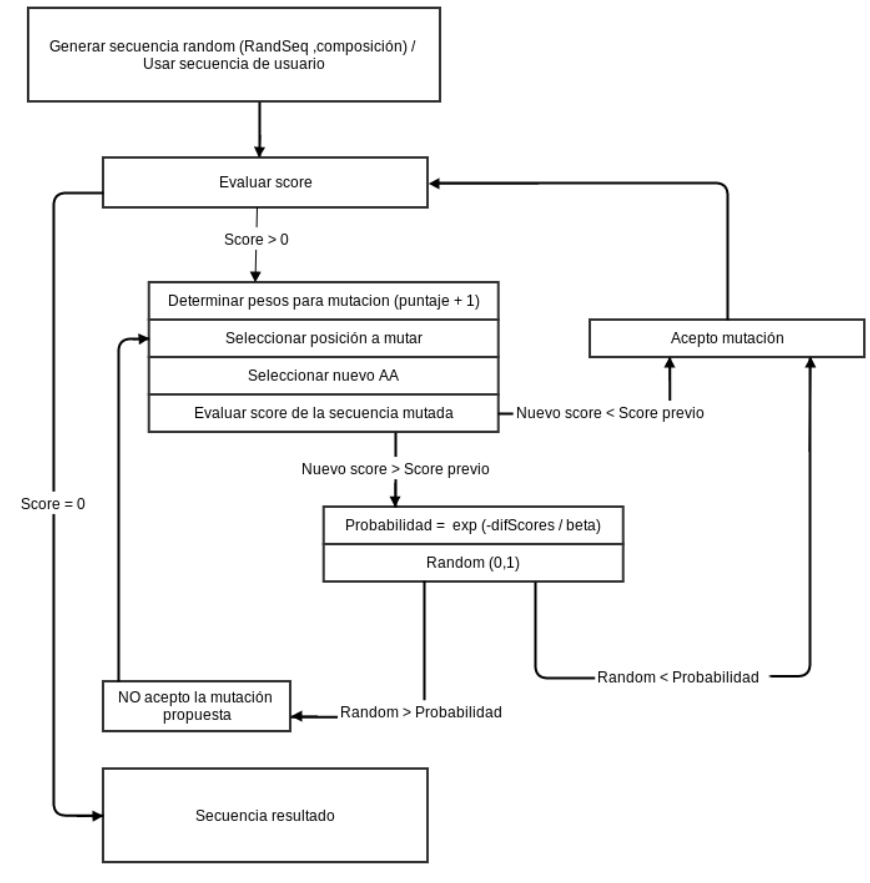
\includegraphics[width=\textwidth]{img/diagrama-algoritmo-2.png}
 \caption{Esquema general del método aplicado para obtener la secuencia final}
 \label{fig:esquema-algoritmo}
\end{figure}



\subsection{Secuencia inicial}\label{seqInicial}

El método comienza a iterar a partir de una secuencia inicial. 
Esta secuencia puede ser creada de forma aleatoria como primer paso del 
algoritmo(ver \ref{secuenciaInicialRandom}) o puede ser pasada como parámetro por el usuario \ref{secuenciaInicialDefinida}. 

La generación de una secuencia aleatoria no es un problema trivial. 
En la naturaleza las proteínas están compuestas de un conjunto de 20 aminoácidos, los cuales se encuentran con diferentes abundancias relativas. 
La frecuencia de cada aminoácido dentro de un proteoma está dada por un balance entre el costo metabólico de este y la necesidad de contar con un conjunto de secuencias diversas que darán proteínas funcionales \cite{krick2014amino}. 
Para generar una secuencia aleatoria, entonces, es necesario definir primero la frecuencia que tendrá cada aminoácido. 
Esta frecuencia se obtiene a partir de la frecuencia global que tiene cada aminoácido en la base de datos de secuencias proteicas.
La aplicación que se utiliza para obtener la secuencia random es RandSeq \cite{randseq}.

Por default, la herramienta utiliza la composición estándar obtenida de SwissProt \cite{compositionAA}.  
Estos valores resultan del cálculo de la composición de aminoácidos de todas las proteínas de la base de datos. 
De esta forma, la composición total representa un consenso de frecuencias de aminoácidos entre todas las secuencias documentadas hasta el momento en la base de datos UniProtKB/Swiss-Prot.
% Los valores de la composición estándar se encuentran en http://web.expasy.org/protscale/pscale/A.A.Swiss-Prot.html

Entre otras que existen, esta herramienta ofrece la posibilidad de definir las frecuencias que desea para cada aminoácido e, incluso,
indicar solo la frecuencia de algunos residuos en particular, dejando el restos con la frecuencia estándar. 
Nuestra herramienta también ofrece al usuario esta flexibilidad para definir la composición que tendrá la secuencia (ver \ref{composicion})
Esta funcionalidad permitiría, por ejemplo, indicar que cierto aminoácido no esté presente en la secuencia (asignándole una frecuencia igual a 0). 
Para el fin que tiene la herramienta, es útil tener este tipo de funcionalidades ya que permite adaptar los requerimientos a las capacidades(limitaciones) del laboratorio experimental. 
El nuevo linker diseñado deberá poder ser sintetizado eficientemente junto con la nueva proteína, lo cual implica una carga metabólica para el sistema biológico en el cual está siendo expresado. 
De esta forma, se intentará adaptar las propiedades de la secuencia diseñada para aumentar la capacidad de síntesis reduciendo, por ejemplo, los aminoácidos que implican un gran gasto energético
y que limitarán la producción de la proteína final.




% \subsection{Método de evaluación de la secuencia}


% Para poder implementar la busqueda guiada por información resultante de evaluaciones secuenciales, primero debemos poder representar esta información de forma concreta/cuantitativa.
% Para esto, de cada evaluación realizada sobre la secuencia se extrae un valor binario para cada posición. Un valor = 1 representa una evaluación negativa con respecto al comportamiento deseado, 
% mientras que un valor = 0 implica una evaluación positiva.
% Por ej: .........
% ARMAR EJEMPLOS CON HERRAMIENTAS SIN ESPECIFICAR EL NOMBRE DE ESTA,ej:  LA EVALUACION DE LA HERRAMIENTA A RESULTA EN..... Y LA HERRAMIENTA B RESULTA EN ...
% Los valores correspondientes a distintas
% Por ej. si al analisis previo le agregamos una evaluacion para....

% Usando este esquema, se deduce simplemente que la posicion que tenga el mayor valor será la que mas se aleja de nuestro objetivo.

% Una de las desventajas(quizás no), de este esquema , es que el metodo esta orientado a realizar evaluaciones que permitan derivar un valor binario para cada posicion de la secuencia. 
% Esto, al parecer, no seria un problema, ya que el resultado deberia poder adaptarse a este esquema.


% Ya que no conocemos la función exacta que determina la relacion entre la secuencia y los valores de puntajes en las distintas posiciones(ni tampoco su superficie funcional),
% no podemos conocer como varía el puntaje asociado si realizamos una modificacion sobre la secuencia
% Ademas, esta variacion del puntaje con la secuencia depende de distintos factores, no solo del conjunto de herramientas/evaluaciones realizadas, sino también de los parámetros utilizados para éstas.
% La implementación de la búsqueda deberá tener esto en cuenta para realizar una busqueda guiada por estos valores.





\subsection{Evaluación y Mutación}\label{evalYmutacion}

% TENIENDO EN CUENTA ESTAS CONSIDERACIONES, EL ESQUEMA QUE USAMOS NOS PERMITE REALIZAR UN NUMERO REDUCIDO DE MUTACIONES YA QUE SE APUNTA A LAS POSICIONES CON MAS CONFLICTO, 
% ADEMAS EL PARAMETRO BETA PERMITE ADAPTAR LA BUSQEUDA A DISTINTAS FORMAS DE LA SUPERFICIE DEL ESPACIO DE SOLUCIONES, LAS CUAL DEPENDE DE LAS CONDICIONES DE LOS PARAMETROS QUE USAMOS(COMPOSICION, THRESHOLDS, HERRAMIENTAS).
% ES DECIR SI LA SUPERFICIE TIENE MINIMOS LOCALES QUE DEBAN SER SUPERADOS, UN VALOR DE BETA MAS ALTO RELAJA LAS RESTRICCIONES PARA
% ACEPTAR MUTACIONES Y POR LO TANTO PERMITE . CUANDO LA SUPERFICIE ES MAS 'PLANA', UN VALOR DE BETA MENOR PERMITE ENCONTRAR LA SOLUCION CON UN MENOR NUMERO DE MUTACIONES(LO QUE NO SIGNIFICA QUE SEA MAS RAPIDO)
% En este caso, la función a optimizar está dada por el resultado de todas las evaluaciones que queremos realizar.


En cada iteración del método se analiza la secuencia utilizando un conjunto de herramientas de evaluación.
Los resultados de cada evaluación serán reflejados en un valor numérico o puntuación asociado a cada posición
(el capítulo \ref{tools} se centra en las propiedades evaluadas y como se aplican las herramientas utilizadas para dar un valor numérico a cada posición). 

El puntaje es inicializado en 0 para todas las posiciones y cada evaluación ejecutada puede aumentar o mantener el valor de manera tal que, 
al finalizar todas las evaluaciones correspondientes, el puntaje de cada posición tendrá un valor mayor o igual a cero.
% El aumento de este puntaje depende de la concordancia que tiene cada posición con las características evaluadas.
En cada evaluación \textbf{se aumenta el puntaje si el residuo en esa posición NO favorece las propiedades deseadas}.
Definimos el puntaje total de la secuencia como la suma de puntajes de cada posición.
Un ejemplo de análisis de la secuencia mediante dos herramientas de evaluación hipotéticas A y B sería: % PONER EJEMPLO PARA QUE QUEDE CLARO
% \rule[0.9cm]{0pt}{0.9cm}

\vspace{0.3cm}
\begin{tabular}{llllllllllllll} 
\hline
Secuencia & \textbf{M} & \textbf{V} & \textbf{L} & \textbf{S} & \textbf{P} & \textbf{A} & \textbf{D} & \textbf{K} & \textbf{T} & \textbf{N} & \textbf{P} & \textbf{D} \\ \hline
Puntaje Inicial & 0 & 0 & 0 & 0 & 0 & 0 & 0 & 0 & 0 & 0 & 0 & 0\\ \hline
Evaluación con herramienta A & 0 & 1 & 1 & 1 & 1 & 0 & 3 & 2 & 5 & 4 & 1 & 0\\ \hline
Evaluación con herramienta B & 0 & 0 & 1 & 1 & 3 & 5 & 1 & 1 & 0 & 2 & 1 & 2\\ \hline
Puntaje global & 0 & 0 & 2 & 2 & 4 & 5 & 4 & 3 & 5 & 6 & 2 & 2\\ \hline
Puntaje total  & 35 \\ \hline
\end{tabular}

\vspace{0.5cm}

% La secuencia linker es solo una parte de la construccion final correspondiente a la proteína quimérica. 
% De esta forma, y dado que muchos aspectos relevantes del diseño dependen del contexto, el algoritmo permite 

Al terminar todas las evaluaciones sobre la secuencia, el puntaje resultante se utiliza para el proceso de mutación.
% POR QUE HACEMOS UNA MUTACION DE A 1 PASO, ES DECIR 1 SOLA MUTACION POR VEZ? 


El proceso de mutación sigue los siguientes pasos:
\begin{enumerate}
 \item En primer lugar se selecciona uno de los residuos de la secuencia como objetivo para realizar la mutación. 
 Esta selección será ponderada. El factor de ponderación utilizado será el valor resultante de sumar 1 al puntaje global asociado a la posición.
 Siguiendo el ejemplo anterior:
 
 \begin{tabular}{lllllllllllll} 
 \hline
Secuencia &  \textbf{M} & \textbf{V} & \textbf{L} & \textbf{S} & \textbf{P} & \textbf{A} & \textbf{D} & \textbf{K} & \textbf{T} & \textbf{N} & \textbf{P} & \textbf{D}\\  \hline
Puntaje global & 0 & 0 & 2 & 2 & 4 & 5 & 4 & 3 & 5 & 6 & 2 & 2\\  \hline
Factor de ponderación & 1 & 1 & 3 & 3 & 5 & 6 & 5 & 4 & 6 & 7 & 3 & 3\\  \hline
\end{tabular}
 
\vspace{0.5cm}
Esta forma de calcular el factor de ponderación implica que nuncá se tendrán factores iguales a cero y, por lo tanto, siempre se podrá seleccionar alguna posición para mutar.

%  Se debe tener en cuenta que, como se mencionó previamente, el valor del puntaje resultante puede ser igual a 0 y, si esto se repite para todas las posiciones, puede ocurrir que ningún residuo sea factible de ser seleccionado, en cuyo caso no se continúa el proceso de mutación. 
   \item El segundo paso, consiste en seleccionar con que aminoácido se sustituirá la posición seleccionada. 
   Esta selección se realiza siguiendo la misma composición que se definió al iniciar la ejecución \ref{composicion}. 
   Dado que la selección del sustituto es independiente del tipo de residuo seleccionado para mutar,
   es posible que el mutado y su reemplazo seleccionado sean iguales. 
   En este caso simplemente se vuelve a seleccionar un sustituto hasta que el resultado sea un residuo distinto al anterior.     
    \item El tercer paso consiste en aceptar o rechazar la mutación propuesta.
    Para realizar esto, primero se vuelve a evaluar el puntaje, analizando todas las características deseadas de la secuencia pero, esta vez, sobre la secuencia que contiene la mutación propuesta.
    Este resultado nos permite saber como se modificarán los puntajes si aceptaramos la mutación. 
    La decisión se toma en base al puntaje total de la secuencia, resultante de sumar los puntajes de cada posición. Si este  \underline{puntaje total disminuye}, entonces \underline{la mutación es aceptada}. 
    Por ejemplo, si evaluamos la posibilidad de mutar la Leucina en la posición 3 por Fenilalanina:
%     PONER EJEMPLO DONDE DISMINUYA EL PUNTAJE TOTAL

\vspace{0.3cm}
       \begin{tabular}{ccccccccccccc}
       \hline
       
	Secuencia previa &  \textbf{M} & \textbf{V} & \textcolor{blue}{L} & \textbf{S} & \textbf{P} & \textbf{T} & \textbf{D} & \textbf{K} & \textbf{T} & \textbf{N} & \textbf{P} & \textbf{D}\\  \hline
	Puntaje global & 0 & 0 & 2 & 2 & 4 & 5 & 4 & 3 & 5 & 6 & 2 & 2\\  \hline
       Puntaje total(previo) & 35 \\ \hline \hline
       Secuencia mutada & \textbf{M} & \textbf{V} & \textcolor{blue}{L} & \textbf{S} & \textbf{P} & \textbf{T} & \textbf{D} & \textbf{K} & \textbf{T} & \textbf{N} & \textbf{P} & \textbf{D}\\  \hline
	Puntaje global  & 0 & 0 & 3 & 1 & 3 & 4 & 4 & 3 & 5 & 6 & 2 & 2\\  \hline
       Puntaje total(posterior) & 33 \\  \hline
      \end{tabular}\\
      
%       \vspace{0.2cm}
    En este caso, la mutación disminuye el puntaje total(33$<$35) y por lo tanto es aceptada, finalizando la iteración.
%     Dado que las evaluaciones pueden depender del contexto en el que se encuentra cada posición, 
    Una mutación puntual puede cambiar el valor del puntaje en esa posición y/o el valor del puntaje correspondiente a otras posiciones. 
    Por lo tanto, como se ve en el ejemplo, para evaluar el cambio se tiene en cuenta el puntaje total y no exclusivamente el de la posición mutada. 
%     Dado que el puntaje es el resultado de un conjunto de evaluaciones diferentes que analizan la secuencia como un todo, 
    
    
    Si la mutación propuesta \underline{\textbf{NO} disminuye el puntaje total} de la secuencia, entonces la mutación se acepta o rechaza \underline{siguiendo el método de decisión de Monte Carlo}. 
    
%     \subitem 
    Este método deriva una probabilidad de aceptación($P_{aceptar}$) a partir de la diferencia entre los puntajes totales resultantes de la secuencia antes($Puntaje_{previo}$) y después($Puntaje_{posterior}$) de la mutación propuesta.
    La \underline{probabilidad de aceptación} resulta de calcular:
    
    \begin{equation}\label{monteCarlo}
    P_{aceptar} =  \frac{(Puntaje_{previo}  - Puntaje_{posterior}) } {\beta} 
    \end{equation}

    
    El valor del parámetro $\beta$ es propio del método y permite ajustar la probabilidad de aceptación según el perfil de evaluaciones realizadas. 
    En el capítulo \ref{results} se analizan en detalle los efectos globales de este parámetro sobre la herramienta y se evalúan los valores óptimos en función del conjunto de herramientas aplicadas(detalladas en el capítulo \ref{tools}).
    Para ejemplificar el método de decisión de Monte Carlo, tomemos el siguiente caso de mutación en donde si propone mutar el ácido aspártico en la posición 7 por ácido glutámico :
    
    %     EJEMPLO DONDE *NO* DISMINUYE EL PUNTAJE TOTAL
      \vspace{0.3cm}
       \begin{tabular}{ccccccccccccc}\hline
	Secuencia previa &  \textbf{M} & \textbf{V} & \textbf{L} & \textbf{S} & \textbf{P} & \textbf{A} & \textcolor{blue}{D} & \textbf{K} & \textbf{T} & \textbf{N} & \textbf{P} & \textbf{D} \\ \hline
	Puntaje global & 0 & 0 & 2 & 2 & 4 & 5 & 4 & 3 & 5 & 6 & 2 & 2\\  \hline
       Puntaje total(previo) & 35 \\ \hline \hline 
       Secuencia mutada  &  \textbf{M} & \textbf{V} & \textbf{L} & \textbf{S} & \textbf{P} & \textbf{A} & \textcolor{blue}{E}& \textbf{K} & \textbf{T} & \textbf{N} & \textbf{P} & \textbf{D}\\  \hline
	Puntaje global & 0 & 0 & 3 & 3 & 4 & 5 & 4 & 3 & 5 & 6 & 2 & 2\\  \hline
       Puntaje total(posterior) & 37 \\ \hline
      \end{tabular}\\
    
    Para este caso $Puntaje_{previo}=35$ y $Puntaje_{posterior}=36$. Usando un valor de $\beta=1.5$ la ecuación \ref{monteCarlo} resulta en $P_{aceptar} = 0.26$.
%     El resultado de la ecuación \ref{monteCarlo} dará un valor de probabilidad en el rango [0,1]. 
    Para aplicar esta probabilidad dentro del método, obtenemos primero un valor \textit{random} en el rango [0,1], si el valor obtenido es menor que el calculado con la ecuación \ref{monteCarlo} entonces se acepta la mutación propuesta, 
    caso contrario esta no es aceptada. 
    En caso de \underline{NO aceptarse} la mutación propuesta el algoritmo vuelve al paso 1, es decir, se vuelve a \underline{intentar una nueva mutación}. 
        
\end{enumerate} 



% De forma resumida, solo se incorporan mutaciones que se traduzcan en una disminución del puntaje total de la secuencia.


Dado que el objetivo final es obtener una secuencia que posea, con cierta probabilidad, todas las características deseadas, 
el algoritmo finaliza cuando el puntaje resultante sea igual a cero, o cuando se cumple alguna de las condiciones especificadas de finalización \ref{condicionFin}. 
% Esto implica que todas las evaluaciones concuerdan con los objetivos buscados en el diseño de la secuencia linker.






